\section{Sigmoid}
The derivation is similar to Linear regression. The plot for the equation:
\[
  \hat{a}(\vec{x})= \frac{1}{1+e^{-(\vec{w}\cdot{}\vec{x}+b)}}
\]

for one dimension is on figure \ref{fig:sigmoid}. By tuning $w$ and $b$  we can find the best fit. 

From now, the output is named $a$ and $\hat{a}$.

The sign of $w$ reflects the line over $y$ axis, the magnitude controls the slope. Again, $b$ translates over $x$.

\begin{figure}[h]
 \centering
 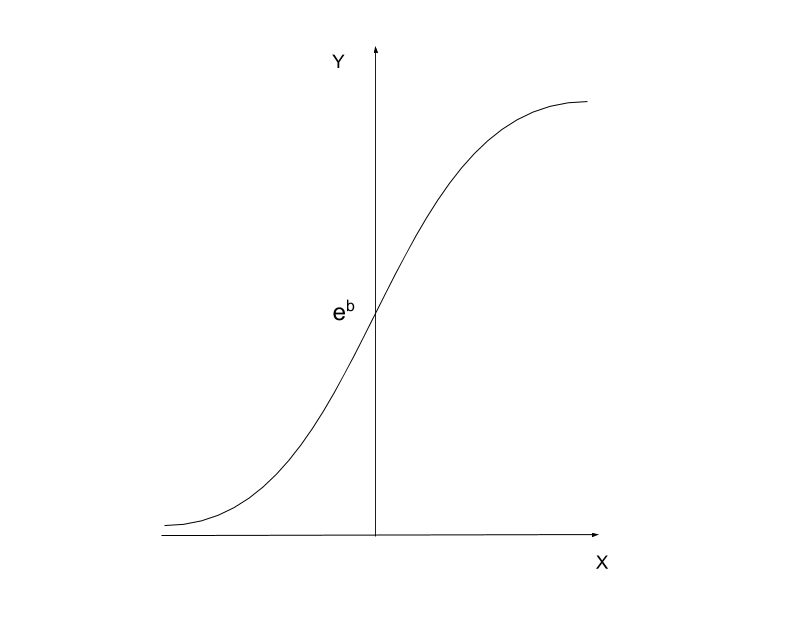
\includegraphics[width=0.9\textwidth]{sigmoid_plot.png}
  \caption{Sigmoid plot} \label{fig:sigmoid}
\end{figure}

\subsection{Forward Propagation}
This step is similar, but with new Loss and $\hat{a}$. 
The Loss is the Cross Entropy Loss.
\begin{align}
  \hat{a}_i &= \frac{1}{1+e^{-(\vec{w}\cdot \vec{x}_i + b)}}\\
  L_i &= a_i\,\log(\hat{a}_i) + (1-a_i)\,\log(1-\hat{a}_i)
\end{align}
Again $\vec{w}\cdot{}\vec{x}_i$ is shorthand for $\sum_{j} w_j\,\mathbf{X}_{ji}$

We calculate cost again:
\begin{align*}
  C(\vec{w}, \vec{b}) &= -\frac{1}{m}\sum_{i=0}^m L_i(\vec{w}, b)
\end{align*}

This is coded:
\begin{verbatim}
1/m*(np.dot(A, np.log(Ap).T) + np.dot(1-A, np.log(1-Ap).T))
#or
1/m*(np.sum(np.multiply(A, np.log(Ap)) + np.multiply(1-A, np.log(1-Ap))))
#tested, yields same number :-)
\end{verbatim}

\subsection{Backward propagation}

\begin{align}
  \frac{\partial L_i}{\partial \vec{w}} = 
  \frac{\partial L_i}{\partial \hat{a}_i}\, \frac{\partial \hat{a}_i}{\partial z}\,\frac{\partial z}{\partial \vec{w}}\\
  \frac{\partial L_i}{\partial b} = 
  \frac{\partial L_i}{\partial \hat{a}_i}\,\frac{\partial \hat{a}_i}{\partial z}\,\frac{\partial z}{\partial b}
\end{align}
The first two derivatives are the same, let's compute them right away. There are many steps, so we won't need any textual explanation.
i
\begin{align*}
  \frac{\partial L_i}{\partial \hat{a}_i} &= \frac{a_i}{\hat{a}_i} + \frac{(1-a_i)}{1-\hat{a}}\,(-1) \\
  \frac{\partial \hat{a}}{\partial z} &= \ldots  \label{eq:derZ}\\
  a(z)&= \frac{1}{1+e^{-z}}\\
  a(u)&=\frac{1}{u}\\
  da&=-u^{-2}\,du\\
  \frac{da}{dz}&=-\left(\frac{1}{1+e^{-z}}\right)^{-2}\,e^{-z}(-1)\\
  &=\left(\frac{1}{1+e^{-z}}\right)^{-2}\,(e^{-z} + 1 -1)\\
  &= \hat{a}^2\,(\frac{1}{\hat{a}} -1) \\
  \frac{\partial \hat{a}_i}{\partial z} &= \hat{a}_i\,(1-\hat{a}_i)
\end{align*}
The last derivative is:
\begin{align*}
  \frac{\partial L_i}{\partial \hat{a}_i}\,\frac{\partial \hat{a}}{\partial z} &= \left[ \frac{a_i}{\hat{a}_i} + \frac{(1-a_i)}{1-\hat{a}}\,(-1) \right]\,\hat{a}_i\,(1-\hat{a}_i)\\
  &= a_i - \hat{a}_i\\
  \frac{\partial z_i}{\partial w} &= x_i\\
  \frac{\partial z_i}{\partial b} &= 1
\end{align*}
We are left with:

\begin{align*}
  \frac{\partial L_i}{\partial \hat{a}_i}\,\frac{\partial \hat{a}}{\partial z}\,\frac{\partial \hat{z}}{\partial \vec{w}} &= \left(a_i - \hat{a}_i\right)\,\vec{x}_i\\
  \frac{\partial L_i}{\partial \hat{a}_i}\,\frac{\partial \hat{a}}{\partial z}\,\frac{\partial \hat{z}}{\partial b} &= \left(a_i - \hat{a}_i\right)\,1\\
\end{align*}
$\vec{x}_i$ are all the features of sample $i$, not just one.
So part of the derivative turns out to be simple to calculate. Using $dw$, $db$ we can update values:

\begin{align}
  w_j &= w_j - \frac{\partial C}{\partial w_j}\,\alpha\\
  &= w_j + \frac{1}{m}\,\sum \frac{\partial L_i}{\partial w_j}\,\alpha\label{eq:same}\\
  \vec{w} &= \vec{w} - \frac{\partial C}{\partial \vec{w}}\,\alpha\\
  b &= b - \frac{\partial C}{\partial b}\,\alpha
\end{align}

When we compute the process involves \ref{eq:same}, and this is the exact same result than for linear regression. 
